Lifetimes of certain brand of switch follows (approximately) a normal distribution with mean 100 hours.  Five switches of a new brand are obtained and tested and their lifetimes measured to be 120, 101, 114, 95, and 130 hours.  Does this provide strong evidence that the new switches have a longer average lifespan?
\begin{mybox}
    \textbf{Solution:} 
    \begin{align*}
        H_0 &: \mu_0 = 100 \text{ hours}
        \\ H_a &: \mu_a > 100 \text{ hours} 
    \end{align*}
    
    The sample mean is $\mu = 112$. The sample standard deviation is
    \begin{align*}
        S^2 &= \dfrac{\sum(x_i-\bar{x})^2}{n-1}\\
        &= \frac{(95-112)^2 + (101-112)^2 + (114-112)^2 + (120-112)^2 + (130-112)^2}{5-1}  \\ &= 200.5
    \end{align*}
    and $S \approx 14.1598$. Then our test statistic is
    $$\mathcal{T} = \frac{\xbar - \mu}{S \big/ \sqrt{n}} = \frac{112-100}{14.1598 \big/ \sqrt{5}} \approx 1.895.$$
    Using an $\alpha = 0.01$ significance level with $n-1 = 4$ degrees of freedom. Via Table 5, $t_{0.005}(4) = 4.604$. The respective $p$ value is
    \begin{align*}
        p &= \Pr(\mathcal{T} \geq 1.895 \mid \mu_0 = 100)\\
        &< \Pr(\mathcal{T} \geq 4.604)\\
        &= 0.005  \tag{WebAssign \say{technology}}\\
        &< \alpha
    \end{align*}
    Hence, we reject $H_0$ and conclude that there is sufficient evidence that the\\ lifespan has increased.
    \noindent \begin{center}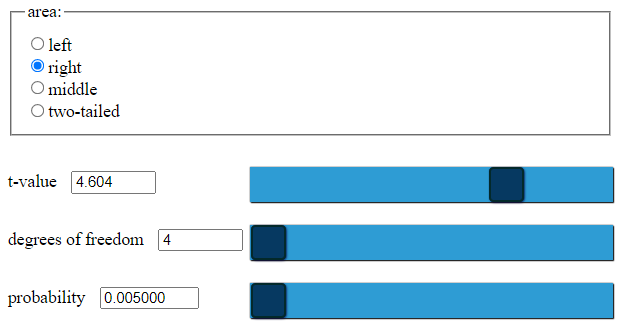
\includegraphics[width=4.5in]{p2.PNG}
    \end{center}
\end{mybox}